\documentclass{article}
\usepackage[utf8]{inputenc}
\usepackage{hyperref}
\usepackage[letterpaper, portrait, margin=1in]{geometry}
\usepackage{enumitem}
\usepackage{amsmath}
\usepackage{booktabs}
\usepackage{graphicx}
\usepackage{hyperref}
\usepackage{titlesec}
\usepackage[section]{placeins}

\hypersetup{
colorlinks=true,
    linkcolor=black,
    filecolor=black,      
    urlcolor=blue,
    citecolor=black,
}

  
\title{Economics 7103 - Homework 2}
\author{Ana Mazmishvili}
\date{ January 29, 2024 }
  
\begin{document}
  
\maketitle 

\section*{Python}
\textbf{Note:} \textit{ While working on this HW, I got help from Afi only with the Python codes.}

\subsection*{Question 1.1}
\textbf{Response:} Randomization worked which is demonstrated by comparison across control and treatment groups that indicates statistical balance in observables. Column 3 presents the differences in means and the standard errors of the differences in brackets. The differences are small and in case of electricity consumption statistically significant.

\begin{table}[hbt!]
    \centering
    \begin{tabular}{lccc}
\toprule
 & Control & Treatment & P-value \\
\midrule
Monthly electricity usage by HHs (kWh) & 1181.33 & 1086.75 & 0.001 \\
  & 454.31 & 423.96 & [3.403] \\
Square feet of home & 1633.05 & 1657.55 & 0.572 \\
  & 682.90 & 686.27 & [-0.566] \\
Outdoor average temperature (\textdegree F) & 79.89 & 79.89 & 0.987 \\
  & 2.16 & 1.97 & [-0.016] \\
Observations & 501 & 499 &   \\
\bottomrule
\end{tabular}

    \caption{Summary Statistics for the treated and control groups.}
    \label{tab:my_label}
\end{table}


\subsection*{Question 1.2}

\begin{figure}[hbt!]
    \centering
    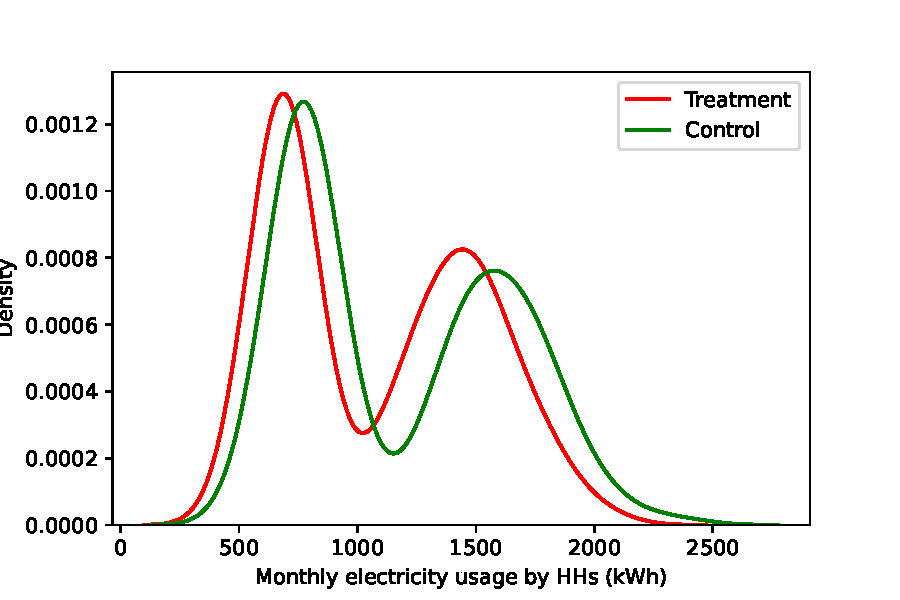
\includegraphics[scale = 0.7]{homework 2/output/figure/densityplotpy.pdf}
    \caption{Kernel density plots of the electricity use for treated group and control group.}
    \label{fig:hist}
\end{figure}


\FloatBarrier
\subsection*{Question 1.3}
(a) I used the Numpy package in Python to create an array X that is the 1000×4 matrix of the predictor variables (3) and a column of ones and an array Y that is the 1000×1 vector
of the dependent variable. The codes are provided in the Python code file. I used matrix operations to calculate \(\hat{\beta}\). Recall that 

\[\hat{\beta} = (X^{'}X)^{-1}X^{'}Y \]

I obtained \(\hat{\beta}\) that is a 4x1 vector with the following values [   0.615 -109.666  3.255 -83.603]

\FloatBarrier
\section*{Stata}

\subsection*{Question 2.1}

I created a table that displays each variable’s sample mean, sample standard deviation, and p-values for the two-way t-test between treatment and control group means. Please see the Table \ref{tab:sum_table}


\begin{table}[hbt!]
    \centering
    {
\def\sym#1{\ifmmode^{#1}\else\(^{#1}\)\fi}
\begin{tabular}{l*{3}{c}}
\hline\hline
            &\multicolumn{1}{c}{Control}&\multicolumn{1}{c}{Treatment}&\multicolumn{1}{c}{P-value}\\
\hline
electricity &    1181.33 &    1086.75 &       0.001\\
            &   (454.31) &   (423.96) &     [3.404]\\
sqft        &    1633.05 &    1657.55 &       0.572\\
            &   (682.90) &   (686.27) &    [-0.566]\\
temp        &      79.89 &      79.89 &       0.987\\
            &     (2.16) &     (1.97) &    [-0.016]\\
\hline
Observations&         501&         499&       1,000\\
\hline\hline
\end{tabular}
}

    \caption{Summary statistics produced using Stata}
    \label{tab:sum_table}
\end{table}

\subsection*{Question 2.2}

I created a two-way scatterplot of electricity consumption and square feet of home data using Stata. Please refer to the Figure below.

\begin{figure}[hbt!]
    \centering
    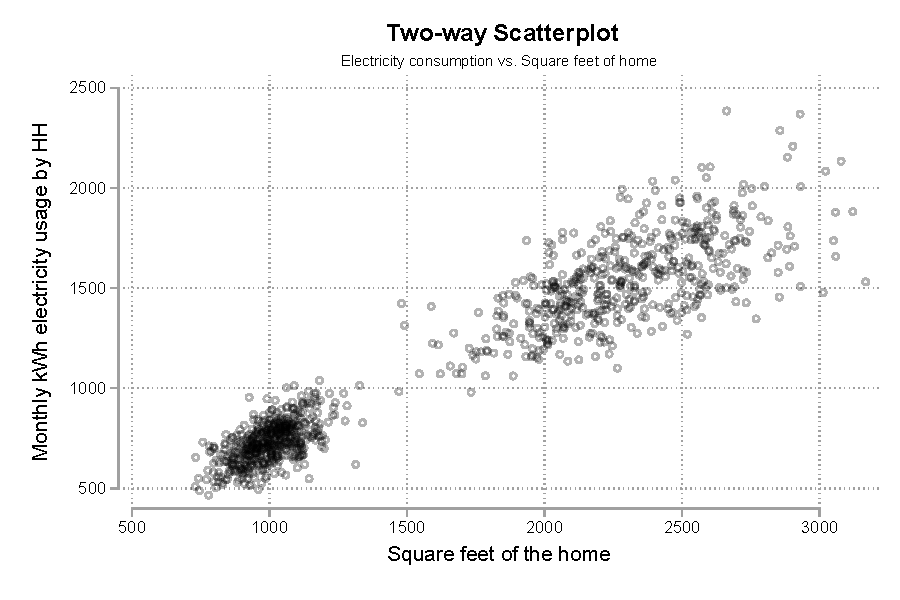
\includegraphics[scale = 0.7]{homework 2/output/figure/scatterplot.pdf}
    \caption{Scatterplot with electricity consumption and square feet of home}
    \label{tab:scatter}
\end{figure}

\FloatBarrier
\subsection*{Question 2.3}
I estimated model using OLS and obtained heteroskedasticity robust standard errors and coefficients. Please refer to the Table below. 

\begin{table}[hbt!]
    \centering
    \documentclass[]{article}
\setlength{\pdfpagewidth}{8.5in} \setlength{\pdfpageheight}{11in}
\begin{document}
\begin{tabular}{lc} \hline
 & (1) \\
VARIABLES & electricity \\ \hline
 &  \\
retrofit & -109.7*** \\
 & (7.943) \\
sqft & 0.615*** \\
 & (0.00678) \\
temp & 3.255* \\
 & (1.932) \\
Constant & -83.60 \\
 & (154.7) \\
 &  \\
Observations & 1,000 \\
 R-squared & 0.919 \\ \hline
\multicolumn{2}{c}{ Robust standard errors in parentheses} \\
\multicolumn{2}{c}{ *** p$<$0.01, ** p$<$0.05, * p$<$0.1} \\
\end{tabular}
\end{document}

    \caption{OLS regression results using Stata}
     \label{tab:robust_table}
  \end{table}




\end{document}